 \chapter{Participa.br: O Portal de Participação Social do Governo Brasileiro}
\label{cap:participabr}

O Participa.br - Plataforma Federal da Participação Social é um espaço colaborativo  para participação social, escuta das demandas do povo e um espaço de dialogo da sociedade com o governo. A imagem ilustrada pela figura~\ref{fig:participabr} apresenta a página inicial do Participa.br

\graphicspath{{figuras/}}
\begin{figure}[H]
\centering
\includegraphics[width=0.9\textwidth]{participa}
\caption{Tela Inicial do Participa.br.}
\label{fig:participabr}
\end{figure}

Ele tem como um dos seus principais objetivos, a criação de um canal de comunicação e participação entre cidadãos e gestores públicos. O Participa.br é uma ação do Gabinete Digital, que é uma iniciativa online do Governo Federal para ampliar o acesso do cidadão à informação pública, serviços, prestação de contas e participação popular nas decisões \cite{gabinete2013brasil}. O Gabinete Digital foi anunciado pela presidenta Dilma Rousseff como resposta às manifestações ocorridas em todo território brasileiro em junho do ano de 2013, e uma de suas principais funções é realizar uma comunicação direta com a sociedade através das redes sociais.

No Participa.br, o cidadão pode se juntar a comunidades com temáticas do seu interesse, como por exemplo, educação, saúde, inclusão digital, entre outras. O Participa.br, permite também que participante crie uma comunidade com o tema de seu interesse, caso não exista. Isso é importante para que os usuários possam utilizar a ferramenta para debater temas que lhe interessem, isto torna a ferramenta mais atrativa. Para isso basta apenas que o usuário crie uma comunidade e alguém que administre ou modere a criação de comunidades na ferramenta do Participa.br aprove a mesma.

Uma das características do Participa.br é servir, além de um espaço de consulta pública, também como uma ferramenta para formulação de novas políticas públicas. Quem acessava a página inicial Participa.br durante os dias 19 de março de 2014 a 17 de abril de 2014, participava de um questionário para definição sobre a definição direitos e princípios fundamentais para garantir o futuro democrático e orientar a governança na internet. O participante respondia 3 perguntas, cada uma com um par de propostas, sem limites de respostas. A cada pergunta o usuário votava na opção que se concordava mais, caso não houvesse nenhuma proposta que ele mais se identificasse ele poderia sugerir novas propostas. O resultado dessa consulta foi enviado como uma Carta Proposta para o Comitê Gestor da Internet, o qual era o gestor do Arena NET Mundial, um evento realizado durante os dias 22 a 24 de abril de 2014 na cidade de São Paulo, com o objetivo de discutir ideias para garantir uma internet livre, colaborativa e democrática \footnote{Maiores informações em: \url{http://www.participa.br/arena}}.

Quando o usuário acessa o Participa.br, ele só pode acessar as ferramentas de participação social, se o mesmo estiver registrado na plataforma. O registro é bem simples, necessitando apenas alguns dados como nome de usuário, senha, nome, e-mail, entre outros. Após o registro um e-mail é enviado para o usuário, este contém o link para ativação do usuário no Participa.br (para evitar criação de spans de usuário). Após a ativação o cidadão já pode fazer comentários e contribuições na plataforma, personalizar o seu perfil, divulgar sua opinião em consultas públicas, manter o seu blog, participar e/ou criar comunidades, etc.

\section{Método de Desenvolvimento do Participa.br}

Estudos realizados em \cite{ferreira2008software} mostram que 40\% de todos os softwares vendidos no Brasil são comprados pelo governo. Esse mesmo estudo mostra a grande influência que o governo exerce sobre as aquisições de software feitas em território nacional, incluindo aquisições de softwares feitas por entidades privadas.

Esse modelo de aquisição de software encontrado nas três esferas do governo ainda se baseia na contratação do melhor fornecedor do software que fornece o melhor atendimento paras necessidades levantadas, essa contratação é feita através do processo licitatório que é o método de aquisição e contratação de produtos que utilizam a verba pública. 

No inicio de uma contratação, geralmente após a identificação da necessidade. Para essa necessidade geralmente é escolhido uma ferramenta já pronta, que é adaptada para a satisfação dos problemas encontrados. Quando o software é colocado em produção é feito o treinamento dos usuários, juntamente com um contrato de manutenção para garantia da correção de bugs, vulnerabilidade e funcionalidades para outras novas necessidades que vão surgindo. Quando se acaba o contrato, muita das vezes a ferramenta é substituída por outra (da mesma empresa ou não), refazendo novamente o ciclo de vida.

Muita das vezes isso acontece, pois a ferramenta é ``fechada‘‘, isto é, somente a empresa que concebeu o software possui o acesso ao código fonte. Isso impossibilita que terceiros possam modificar o código fonte, tornando a compra de uma nova ferramenta uma realidade, sempre que for necessário atender novas necessidades encontradas. Isso gera grande o uso público do dinheiro desnecessariamente.

A Secretaria Geral da Presidência da República \footnote{Disponível em: \url{http://www.secretariageral.gov.br/}}(SGPR) por meio do projeto Participa.br, buscava criar um legado dentro de um software, e ser pioneira em relação a evolução de um software livre por uma entidade governamental. Durante o período de escolha da ferramenta que seria o núcleo do portal de Participação Social, foi procurado uma ferramenta que além de satisfazer as necessidades demandadas para a construção do Participa.br, também seguisse os princípios do Software Livre (visto na seção \ref{sub:softwarelivre}). Ou seja, na medida que o Participa.br vai sendo desenvolvido, sua plataforma de desenvolvimento, o Noosfero (discutido no capítulo \ref{cap:noosfero} também acompanha esse desenvolvimento, algo que ainda é pioneiro nas esferas governamentais.

\subsection{Software Livre}
\label{sub:softwarelivre}

Uma das premissas básicas para a criação do portal de Participação Social Participa.br é em relação a plataforma o qual seria concebida, a primeira regra é que  o software deveria ser livre.

O Software livre permite aos usuários utilizarem, estudarem, modificarem e realizar a distribuição do mesmo, sem restrições e permitindo aos usuários futuros utilizarem de forma igual \cite{bucher2013rede}. Meirelles \citeyear{meirelles2013metricas} mostra que o ecossistema do software livre permite a liberdade dos usuários em relação ao uso do mesmo, sem discriminação de uso, de modo colaborativo e processo de desenvolvimento aberto. Esse ecossistema é o responsável pela diferenciação do software dito restrito para o software livre. O ecossistema do software livre é basicamente um resumo dos quatro direitos básicos de liberdade do software livre aos seus usuários~\footnote{Retirado de \url{http://www.gnu.org}. Acesso em Maio de 2014}:

\begin{itemize}
	\item A liberdade para utilização do software de acordo com o desejo do usuário.
	\item A liberdade para o entendimento do funcionamento do software, e adaptá-lo de acordo com as suas necessidades \footnote{Para satisfazer esse direito de liberdade, o código-fonte do software é um produto indispensável para o mesmo. \label{ft:codfonte}}.
	\item A liberdade de redistribuição do software para qualquer pessoa.
	\item A liberdade para evoluir o software, e distribuir as evoluções feitas para o público em geral, de forma a beneficiar todos os utilizadores do mesmo \footref{ft:codfonte}.
\end{itemize}

Como dito anteriormente, uma das vantagens do software livre é o fato de seu código fonte ser disponibilizado e consequentemente compartilhado \cite{bucher2013rede}. Esse é um dos fatores que contribuem para adaptação de um software para um determinado cenário, sem a necessidade de começar um novo projeto. No Participa.br esse fato é importante pois as contribuições realizadas na ferramenta, ajudam no desenvolvimento tanto do Particpa.br, como da ferramenta em si utilizada.

No Participa.br outro fator interessante para a utilização de um software livre é a propriedade intelectual de todos os conteúdos presentes na ferramenta, fator muito importante se tratando de uma ferramenta governamental, visto que a transparência das informações é algo bastante imprescindível nos dias atuais. Em softwares proprietário geralmente são assinados termos de compromisso e conduta, fazendo com que a empresa proprietária do software acabe se tornando a dona de todas as informações da rede social.

\section{Ferramentas de Participação Social}

De acordo com \cite{solagna2014metodologias} o desenho para um portal como o Participa.br não pode ser algo fechado, ou seja, uma plataforma que oferece todas as formas de participação digital de maneira acabada, mas sim fazer com que os atores da sociedade civil utilizem as ferramentas necessárias para fazer o seu modo de participação, lógico dentro das possibilidades oferecidas pelo Participa, isso aumenta possibilidades de influência nas políticas públicas e nas decisões do Estado. Podemos descrever o Participa.br como um arcabouço de ferramentas de participação onde é possível acoplar novas ferramentas e metodologias de participação de acordo com a necessidade de cada gestor.

A imagem ilustrada pela figura \label{fig:arquiteturaparticipa} possui a atual arquitetura de funcionamento dos mecanismos de participação presentes no Participa.br. O funcionamento de cada ferramentas é discutida mais detalhadamente no   apêndice \label{Att:ferramentasparticipacao}.

\graphicspath{{figuras/}}
\begin{figure}[H]
	\centering
	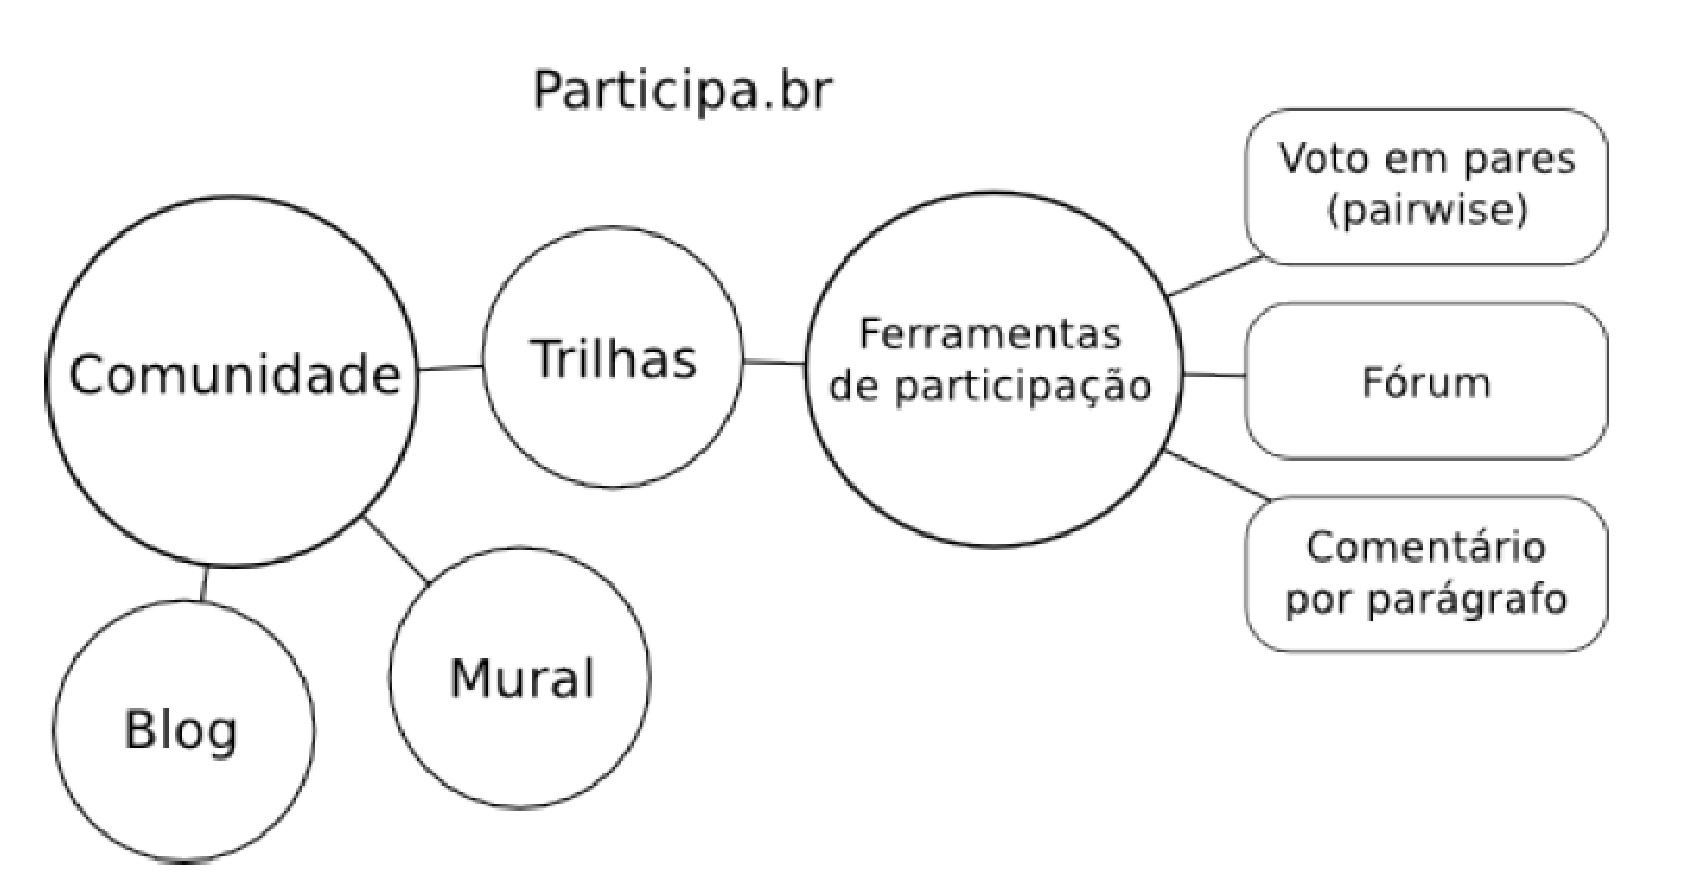
\includegraphics[width=0.7\textwidth]{arquitetura-ferramentas-participa}
	\caption[Atual quadro de ferramentas de participação.]{Atual quadro de ferramentas de participação. Extraído de \cite{solagna2014metodologias}}
	\label{fig:arquiteturaparticipa}
\end{figure}

















